\documentclass[hyperref={unicode}, 14pt, aspectratio=169]{beamer}

\sloppy

% Нумерация формул, таблиц и картинок относительно глав.
\EqInChapter
\TableInChapter
\PicInChapter

% Гипертекстовое оглавление.
\usepackage[
    bookmarks=true,  colorlinks=true, unicode=true,
    urlcolor=black,  linkcolor=black, anchorcolor=black,
    citecolor=black, menucolor=black, filecolor=black,
]{hyperref}

\AfterHyperrefFix

\usepackage{graphicx}
\graphicspath{{assets/}}

% Поля.
\geometry{right=20mm, top=20mm, bottom=20mm, left=30mm}

\usepackage{tikz}
\usetikzlibrary{arrows, arrows.meta, positioning, shadows}

\usepackage{pgfplots}
\pgfplotsset{compat=1.12}

\usepackage{enumerate}
\usepackage{multirow}
\usepackage{paralist, array}
\usepackage{fancyvrb}
\usepackage{changepage}
\usepackage{colortbl}

% Центрирование подписей.
\usepackage[justification=centering]{caption}
\usepackage{subcaption}

\usepackage{totcount}
\newtotcounter{citnum}
\def\oldbibitem{} \let\oldbibitem=\bibitem
\def\bibitem{\stepcounter{citnum}\oldbibitem}

\newcommand{\vect}[1]{\boldsymbol{\mathbf{#1}}}

\newenvironment{conditions}[1][где]
    {#1 \begin{tabular}[t]{l @{~--- } l}}
    {\end{tabular}\\[\belowdisplayskip]}

\newenvironment{definition}[1]
    {\noindent#1\begin{adjustwidth}{.5\parindent}{}\noindent\ignorespaces}
    {\end{adjustwidth}}


\title{Метод ранжирования информационных источников по степени доверия}
\author[Павелко Павел Юрьевич]{Выполнил: Павелко Павел Юрьевич, ИУ7-81 \\ Руководитель: Бекасов Денис Евгеньевич, ИУ7}
\institute[]{МГТУ им. Баумана}
\date{Москва, \the\year}

\begin{document}

\begin{frame}
  \titlepage
\end{frame}

\begin{frame}
    \begin{block}{Цель}
        Разработка системы мониторинга новостей с последующим ранжированием источников по степени доверия
    \end{block}

    \begin{block}{Задачи}
        \begin{enumerate}
            \item Проанализировать предметную область
            \item Разработать метод ранжирование источников
            \item Разработать программное обеспечение
            \item Исследовать применимость метода
        \end{enumerate}
    \end{block}
\end{frame}

\begin{frame}
    \frametitle{Актуальность}

    \begin{block}{}
        \begin{enumerate}
            \item Более 100 тыс. новостных сообщений ежедневно от почти 7 тыс. значимых источников
            \item Достоверность новостей вызывает сомнения
            \item Эксперты способны проверить лишь новости популярных источников
        \end{enumerate}
    \end{block}

    \begin{block}{Вывод}
        Необходим метод распространения оценки эксперта на схожие новости менее популярных источников с последующим ранжированием источников по степени доверия
    \end{block}
\end{frame}

\begin{frame}
    \frametitle{Постановка задачи}

    \begin{center}
        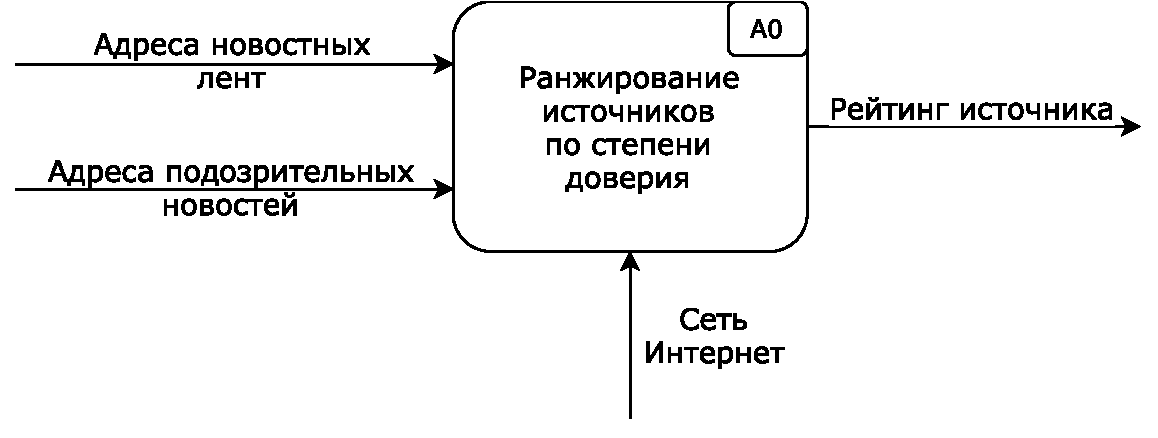
\includegraphics[width=\linewidth]{common.pdf}
    \end{center}
\end{frame}

\begin{frame}
    \frametitle{Предложенный метод}

    \begin{center}
        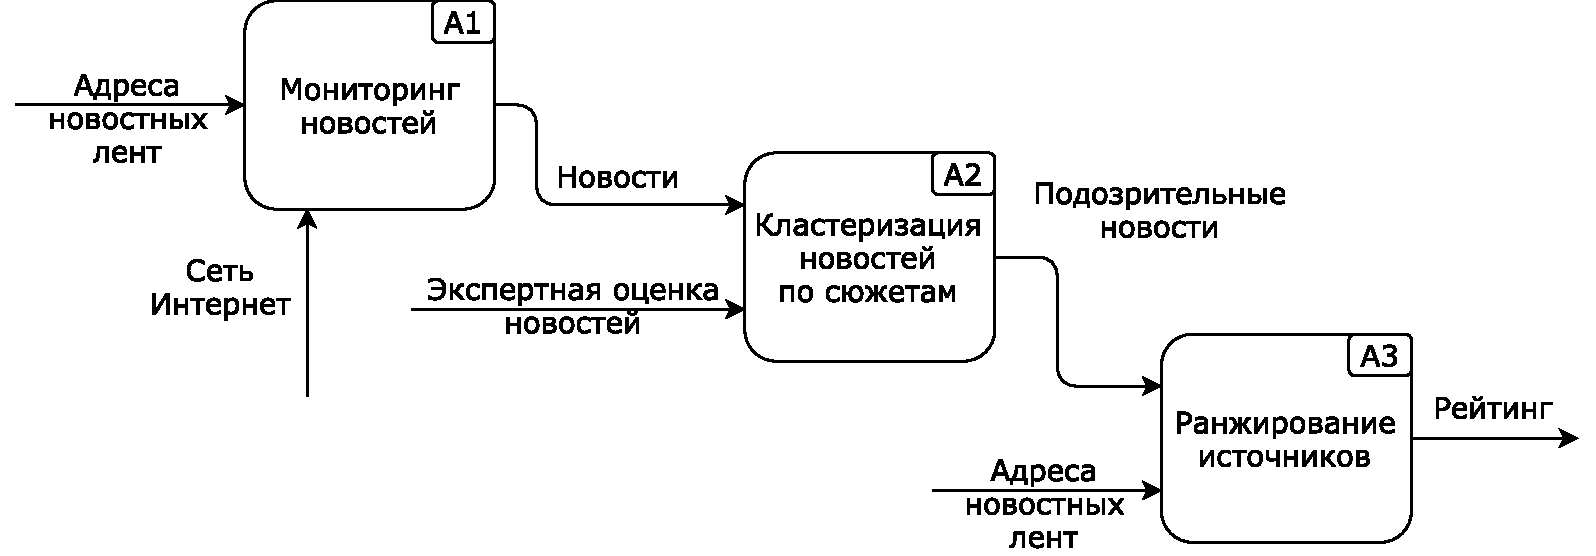
\includegraphics[width=\linewidth]{stages.pdf}
    \end{center}
\end{frame}

\begin{frame}
    \frametitle{Потоки данных в системе}

    \begin{center}
        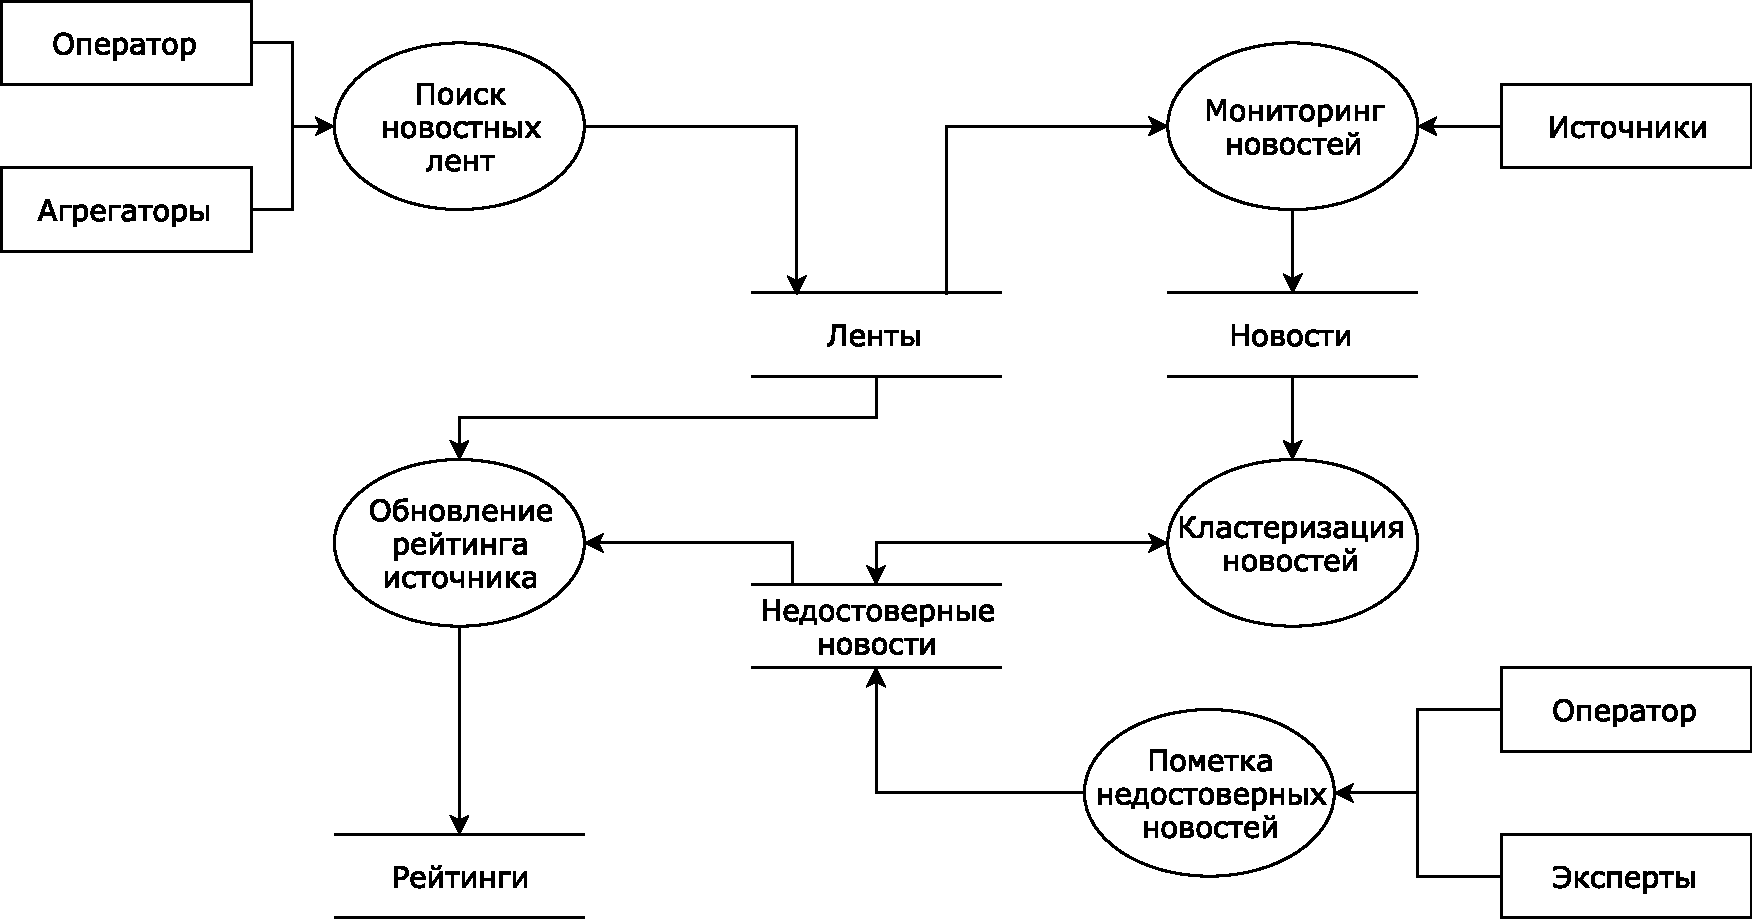
\includegraphics[width=.9\linewidth]{dataflows.pdf}
    \end{center}
\end{frame}

\begin{frame}
    \frametitle{Мониторинг новостей}

    \begin{center}
        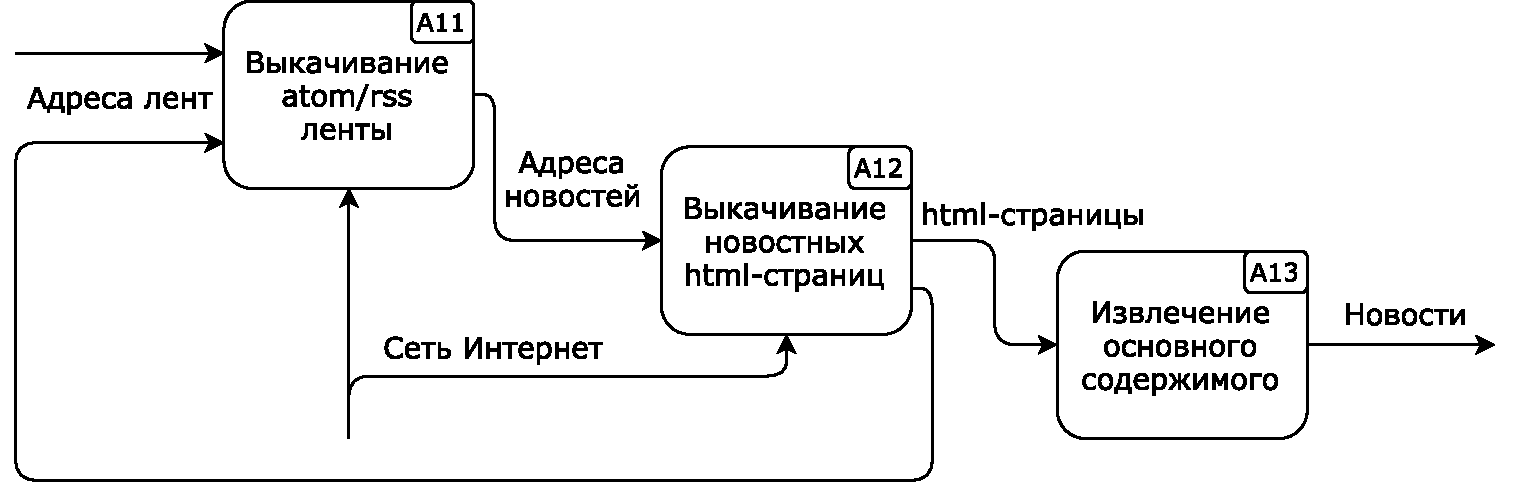
\includegraphics[width=\linewidth]{raider.pdf}
    \end{center}
\end{frame}

\begin{frame}
    \frametitle{Извлечение содержимого}

    \begin{block}{Readability Algorithm}
        \begin{enumerate}
            \item Оценка узлов DOM-дерева по различным показателям
            \item Ранжирование узлов по оценке
            \item Извлечение текстового содержимое наиболее значимых узлов
        \end{enumerate}
    \end{block}

    \begin{block}{Основные показатели}
        \begin{itemize}
            \item Длина текста и доля ссылок в тексте
            \item Количество запятых в тексте
            \item Доля изображений, списков и т.д.
            \item Классы, идентификаторы и теги
        \end{itemize}
    \end{block}
\end{frame}

\begin{frame}
    \frametitle{Кластеризация новостей}

    \begin{center}
        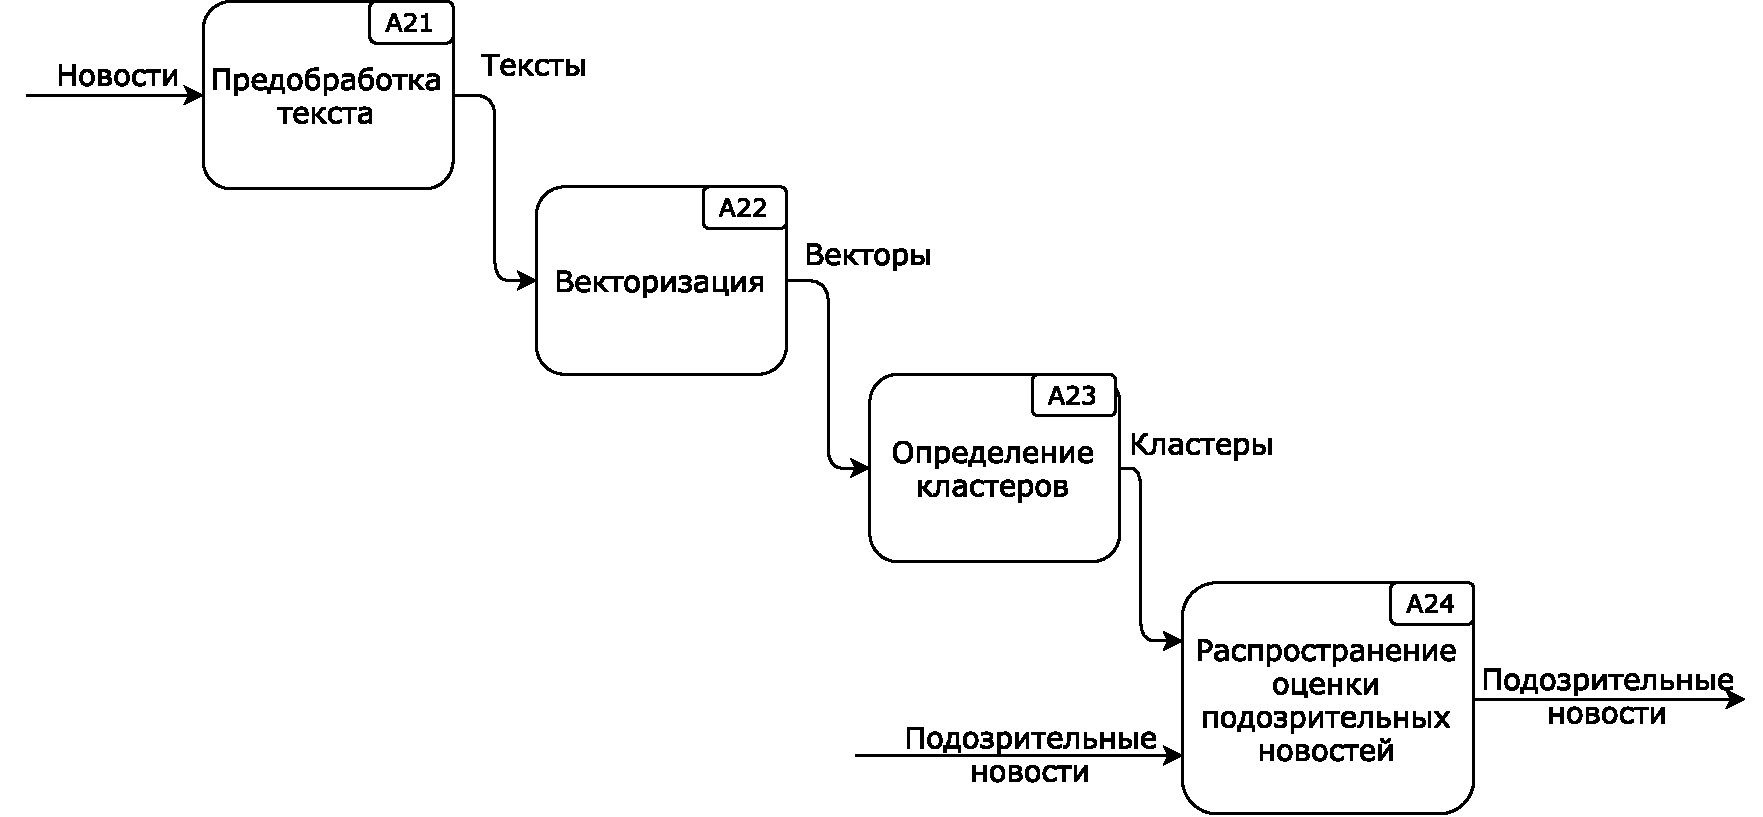
\includegraphics[width=\linewidth]{compounder.pdf}
    \end{center}
\end{frame}

\begin{frame}
    \frametitle{Выбор алгоритма кластеризации}

    \begin{block}{}
        \begin{center}
            \begin{tabular}{ l | l | l | l | >{\columncolor[gray]{0.8}} l }
                \hline
                & k-m & HAC & DHCA & ICA \\ \hline
                Адаптивное кол-во кластеров & $-$ & $+$ & $+$ & $+$ \\ \hline
                Иерархические кластеры & $-$ & $+$ & $+$ & $-$ \\ \hline
                Онлайновый алгоритм & $-$ & $-$ & $+$ & $+$ \\ \hline
                Возможность оптимизаций & $-$ & $-$ & $-$ & $+$ \\
                \hline
            \end{tabular}
        \end{center}
    \end{block}

    \begin{block}{Алгоритмы}
            k-m~--- K-means

            HAC~--- Hierarchical Agglomerative Clustering

            DHC~--- Dynamic Hierarchical Compact Algorithm

            ICA~--- Incremental Clustering Algorithm
    \end{block}
\end{frame}

\begin{frame}
    \frametitle{Incremental Clustering Algorithm}

    \begin{columns}
        \begin{column}{0.35\textwidth}
            Добавление новости:
            \begin{center}
                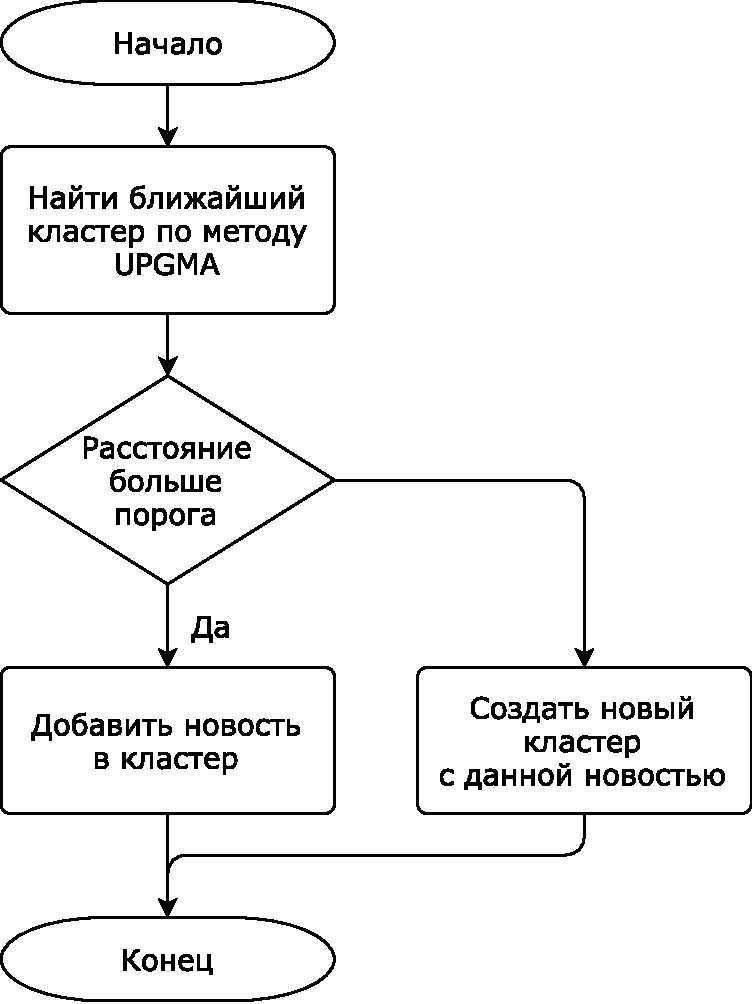
\includegraphics[height=.7\textheight]{ica.pdf}
            \end{center}
        \end{column}
        \begin{column}{0.65\textwidth}
            UPGMA:

            \[
                upgma(C_i,C_j)=\frac{1}{|C_i||C_j|}\sum_{\mathbf{x}\in C_i}\sum_{\mathbf{y}\in C_j}sim(\mathbf{x},\mathbf{y}),
            \]
            \begin{conditions}
                $C_i, C_j$ & кластеры \\
                $\mathbf{x}, \mathbf{y}$ & новости как <<мешки слов>> \\
                $sim(\cdot, \cdot)$ & мера схожести новостей: \\
            \end{conditions}

            \[
                sim(\mathbf{x},\mathbf{y})=\mathbf{x}\mathbf{y}\cdot(1-penalty(x,y))
            \]
        \end{column}
    \end{columns}

\end{frame}

\begin{frame}
    \frametitle{Ранжирование источников}

    \begin{center}
        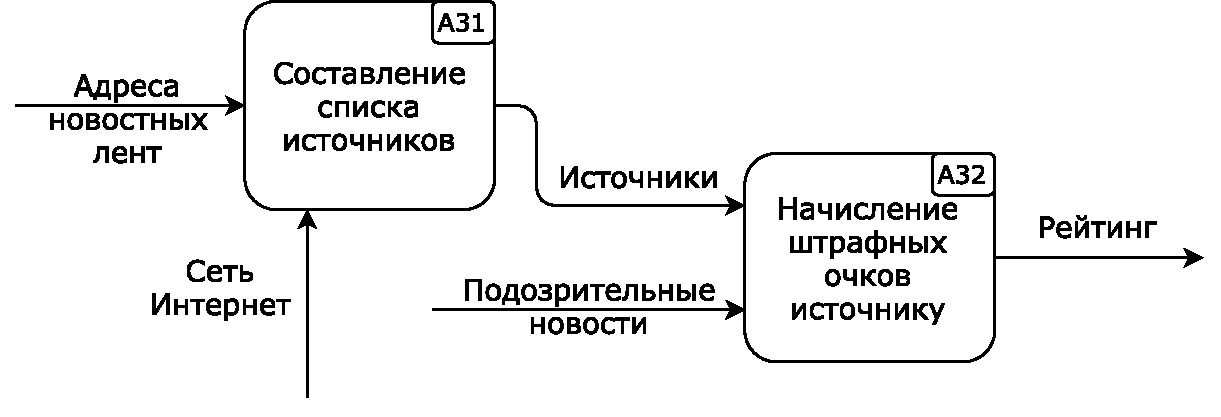
\includegraphics[width=\linewidth]{rater.pdf}
    \end{center}
\end{frame}

\begin{frame}
    \frametitle{Исследование влияния выбора меры сходства на качество кластеризации}

    \begin{block}{}
        TODO

        \begin{enumerate}
            \item постановка
            \item цель
            \item размер выборки
        \end{enumerate}
    \end{block}
\end{frame}

\begin{frame}
    \frametitle{Выводы из работы}

    \begin{block}{}
        \begin{enumerate}
            \item Проанализирована предметная область
            \item Разработан метод ранжирования источников
            \item Разработано программное обеспечение
            \item Исследована применимость метода
        \end{enumerate}
    \end{block}
\end{frame}

\begin{frame}
    \frametitle{Дальнейшее развитие}

    \begin{block}{}
        \begin{itemize}
            \item Построение тематического рейтинга источников
            \item Агрегированная экспертная оценка
            \item Ранжирование экспертов
            \item Нахождение дубликатов и определение первоисточника
            \item Связывание сюжетов по тематике
        \end{itemize}
    \end{block}
\end{frame}

\end{document}
